\documentclass{article}
\usepackage {inputenc, fullpage, listings, amsmath, graphicx, amssymb, xcolor}

\parindent 0pt

\title{%
   CSc 320: Foundations of Computer Science (Summer 2022)\\
    \Large Alex Holland\\
    Assignment 5\\
    }
\date{}

\begin{document}

\maketitle

{\bf Question 1}\\
We want to show that $L = \{ \langle A \rangle | A \text{ is a DFA over} \sum^* \text{ and } L(A) = \sum^* \}$ is decidable by giving a high-level description of a decider $M$ with $L(M)=L$. We can design a TM for the given DFA that run finitely and halts.\\

$L$ accepts all strings including the empty string, therefore the TM must accept all
strings and reject none.\\

\begin{center}
    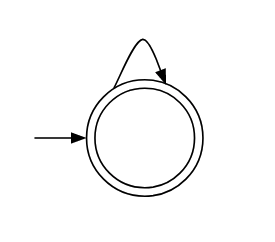
\includegraphics[width=0.2\textwidth]{1.png}
\end{center}

$Y=$ "On input $\langle A \rangle$ where $A$ is a DFA:
\begin{enumerate}
  \item Mark the start state of A
  \item Repeat until no new states are marked\\ - Mark any state that has an incoming transition from a marked state
  \item If any accept state is marked, accept, otherwise, if unmarked, reject"
\end{enumerate}

Since in the constructed DFA there is only 1 state which is also an accept state, all strings are accepted. Only an empty set will be rejected. By step 2 guarantees the DFA will halt because the TM will eventually run out of states to mark.\\

$EQ_{DFA} = \{ \langle A, B \rangle | \text{A,B are DFA's and } L(A) = L(B)$\\

All word in $L(A)$ are in $L(B)$ and there is no word that isn't\\
$L(A) \cup L(B) \neq \emptyset$\\
$\overline{L(A)} \cup \overline{L(B)} = \emptyset$
if and only if $L(A) = L(B)$

We now need to create a DFA that recognizes exactly $L(C) = \overline{L(A)} \cup \overline{L(B)} = \emptyset$. Since $L(C)$ is regular we can construct such DFA that recognizes $L(C)$.\\

$Z=$ "On input $\langle A,B \rangle$ where $A,B=DFA$
\begin{enumerate}
  \item Construct C as show previously 
  \item Simulate TM Y on input $\langle C \rangle$ where Y is the TM that decides $EQ_{DFA}$
  \item If Y accepts, accept. Reject if Y rejects.
\end{enumerate}

Thus, $L = \{ \langle A \rangle | A \text{ is a DFA over} \sum^* \text{ and } L(A) = \sum^* \}$ is decidable.

\break
{\bf Question 2}\\
{\bf a)}\\
The language $L_{min}$ for Minimal DFA Recognition recognizes a DFA $M$ such that there does not exist any other DFA $M'$ that has less states than $M$ for the language $L_{min}$.\\

{\bf b)}\\
We to show that the problem is decidable, in other words, we want to describe a Turing machine that recognizes $L_{min}$. The proof from lecture for DFA state minimization states that if there is a pair $\{p, q\}$ such that $\{\delta(p,a),\delta(q,a)\}$ for some $a \in \sum$, such that $\{p, q\}$ can be removed, since $p \sim q$.\\

We want to create a TM that can run both finitely and recognizes $L_{min}$ which would then prove that $L_{min}$ is decidable.\\

$M =$ "On input $\langle L_{min} \rangle$, where $L_{min}$ is a DFA:
\begin{enumerate}
  \item Remove states that are unreachable
  \item Collapse states for unmarked pairs $\{p, q\}$ if $\{\delta(p,a),\delta(q,a)\}$  is marked for some $a \in \sum$.
  \item If the DFA has been minimized or been has not changed after minimization, accept. Otherwise, reject."
\end{enumerate}

\bigskip
$N=$ "On input $\langle L_{min} \rangle$ where $L_{min}=$ DFA:
\begin{enumerate}
  \item Simulate the TM $M$ on input $\langle L_{min} \rangle$ where $M$ is the TM that decides the minimization of the DFA.
  \item If $M$ accepts, accept. Else reject if $M$ rejects."
\end{enumerate}

\bigskip
Thus, the problem is decidable.\\

\bigskip
{\bf Question 3}\\
We want to show that $L_{\beta}$ is undecidable, where\\ 
$L_{\beta} = \{ \langle M \rangle | \text{ at some point during its computation on empty input } \epsilon, \; M \text{ writes the symbol } \beta \text{ on its tape }\}$. We can do this by using a reduction from $A_{TM}$ to $L_{\beta}$.\\

Note that $A_{TM} = \{ \langle M, w \rangle | M \text{ is a TM and } M \text{ accepts } w \}$\\

Assume $L_B$ is decidable and that there exists some decider $R$ that decides it.\\

Let $S$ be a decider.\\

$S =$ "On input $\langle M, w \rangle$"
\begin{enumerate}
   \item Construct a TM $M'$ as follows:
   \begin{enumerate}
        \item $M'=$ "On input string $x$
        \begin{enumerate}
            \item  If $x \neq \epsilon$, reject
            \item If $x = \epsilon$, run $M$ on $x$. Write $\beta$ to the tape if $M$ accepts, and accept, otherwise, don't write $\beta$ and reject.
        \end{enumerate}
   \end{enumerate}
   \item Run $R$ on input $\langle M' \rangle$
        \begin{enumerate}
            \item If $R$ accepts, accept
            \item If $R$ reject, reject
        \end{enumerate}
 \end{enumerate}
 
Since $S$ is a decider for $A_{TM}$; $R$ only accepts if $M'$ writes a $\beta$ to the tape iff $M$ accepts the input string $x$. Likewise, If $R$ rejects, then it means that $M'$ does not write $\beta$ to the tape if $M$ rejects the input string $x$. Since, a decider has been created for $A_{TM}$, this shows a contradiction, hence, it is proved that $L_{\beta}$ is undecidable. \\

\bigskip
{\bf Question 4}\\
{\bf a)}\\
The language $L_{long}$ for Long Enough Cycle accepts undirected simple graphs that contain a simple cycle with at least $k$ vertices, where none of the vertices except the start and end vertex can be repeated. The cycle is not simple if it has $k$ vertices which can be further broken down into more cycles. We can define the language $L_{long}$ as follows:\\

$L_{long} =\{ \langle G, k \rangle \} | \; G \text{ is a graph such that it contains a simple cycle with at least } $k$ \text{ vertices } \}$\\

{\bf b)}\\
We want to show that Long Enough Cycle is in NP. To prove this, a polynomial verifier that satisfies the definition of a verifier for $L_{long}$ can be given.\\

$\langle G, K \rangle$ is a subset of the Graph G and is a simple cycle with a at least a minimum of $k$ vertices. Let $c$ be the simple cycle used in the following:\\


$V=$ "On input $\langle \langle G,K \rangle, c \rangle$
\begin{enumerate}
    \item Test if c contains edges from one vertex to the next 
    \item Test if $c$ contains repeated vertices
    \item Test if a simple cycle in $c$ contains $\geq k$ vertices
    \begin{enumerate}
       \item Traverse through each vertex, incrementing a counter for each visited vertex, once the end vertex has been reached. Then compare the vertice count in the cycle to $k$
    \end{enumerate}
    \item Test if a cycle is completed in $c$
    \begin{enumerate}
        \item Traverse through each vertex, mark each vertex until the final vertex is reached, check that no other unmarked vertexes can be reached in $c$.
    \end{enumerate}
    \item If all tests pass, accept. Otherwise, reject."
\end{enumerate}


Since traversing through each vertex in the certificate takes linear time for each test, we can say that $V_{long}$ is a polynomial time verifier. Thus, by showing a polynomial verfier for $V_{long}$ with its corresponding certificate, Long Enough Cycles is in $NP$.

\break
{\bf Question 5}\\
We want to prove Sudoku is in $NP$, where empty cells in the Sudoku grid be completed such that each row, each column, and each block contains each integer from $\{ 1, 2, ..., n^2 \}$. In this proof a block, column, and row are represented as follows: \\

The following is an example of a Sudoku grid with prefilled numbers and indication of of it rows, columns and blocks.\\

\textcolor{red}{red }$=block$\\
\textcolor{blue}{blue }$=column$\\
\textcolor{green}{green }$=row$\\

\begin{center}
    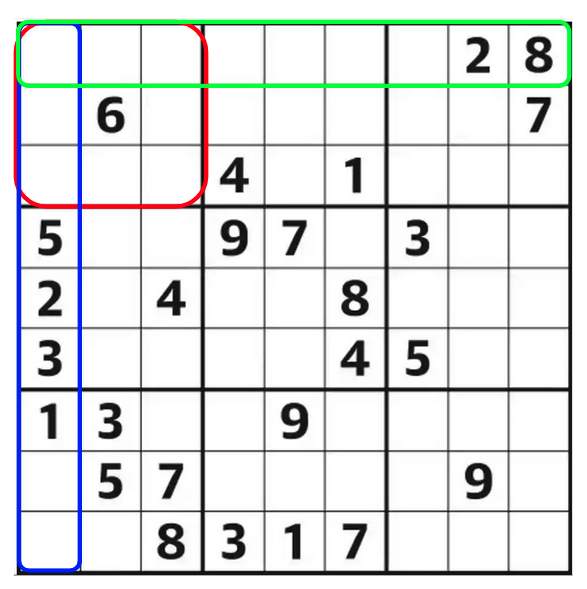
\includegraphics[width=0.6\textwidth]{5.png}
\end{center}

To prove Sudoku is in $NP$, we need to show that Sudoku is both NP-hard and NP-complete.\\

The input size of Sudoku is a finite grid of $n^2 \times n^2$ squares where each of it's column, row, and $n \times n$ block contains $1 \rightarrow n^2$ integers once, they each have fixed a number of solutions depending on the number of squares filled in prior to solving the Sudoku. As such, any $n^2 \times n^2$ grid can be solved in constant time.\\

To prove Sudoku is in NP, a polynomial time verifier, $V_{sudoku}$, can be constructed to check if a solution is valid by verifying that each row, column, and $n \times n$ block has distinct $1 \rightarrow n^2$ integers. The solution is rjected if duplicates are identified in any of corresponding rows, columns, or blocks.\\

A certificate for $V_{sudoku}$ can be described where each row, column, and $n \times n$ block contain unique integers $1 \rightarrow n^2$.\\

Thus with the use of a polynomial verifier $V_{sudoku}$ and certificate, Sudoku is in $NP$.


\end{document}
